\documentclass[12pt,runningheads]{article}
\usepackage[utf8]{inputenc}
\usepackage{graphicx}
\usepackage[left=3.5cm,bottom=4cm]{geometry}
\usepackage[all]{xy}
\usepackage{amsmath,amsthm,amssymb,color,latexsym, mathrsfs, soul}
\usepackage[round]{natbib}
\usepackage{geometry}        
\geometry{letterpaper}    
\usepackage{float}
\setlength{\parskip}{1em}
\usepackage{threeparttable}
\usepackage{lscape}
\usepackage{setspace}
\usepackage{hyperref}
\usepackage{caption}
\usepackage{breqn}
\usepackage{adjustbox}
\usepackage{natbib}

\newcommand\fnote[1]{\captionsetup{font=small}\caption*{#1}}


\title{Family connections and teacher performance: Evidence from Colombian public schools}
\author{Camila Ayala and Juan Felipe Riaño}
\date{October 1, 2022}
\maketitle

\begin{abstract}
    We use data on public school teachers to study the effect of family connections on student's test scores. We consider four different types of family connections: with a non-elected bureaucrat in the public sector, with a council member in the municipality, with a member of the school administration, and with any other teacher within the school. These type of connections vary in both the level influence the family member has on teacher's outcomes and on whether they have an horizontal or vertical relationship. We find that the effect of family connections depends on these factors. First, we find a negative effect on test scores when the relationship between the family member and the teacher is vertical and the family member has a lot of discretion on teacher's career. Second, we find strong and positive effects when the relationship is horizontal and family members have no influence over teacher's careers. The effect is stronger when the connection is to a teacher in the same area or with more experience. The latter suggest that there are positive externalities of working with a family member.
\end{abstract}


\onehalfspacing
\begin{document}
\hypersetup{
    colorlinks=true,
    linkcolor=blue,
    filecolor=blue,      
    urlcolor=blue,
    pdftitle={Overleaf Example},
    pdfpagemode=FullScreen,
    }
    
    


\newpage
\section{Introduction} 

Economists have largely debated the role of family ties at work. There are multiple ways in which family ties can affect worker's outcomes and overall productivity. First, family members can directly affect the hiring and promotion of relatives. Second, family ties can play an important role at job referrals and the likelihood of getting a job. And third, it can affect the worker's performance and overall productivity. Overall, the consensus is that family ties are good for the workers: they help them to get job referrals, get hired, increase their wages, and get promotions (\Citealp{Riano2021}, \Citealp{brassiolo2021}, \Citealp{Manacorda2020}, \Citealp{kramarz2014}, \Citealp{Beaman2012}, \Citealp{ashraf2018}). Nevertheless, the effect of family ties at work on worker's and overall productivity  is ambiguous. The effect would depend on the level of discretion the family member has on the worker's career outcomes, and whether they are peers (horizontal relationship) or in a principal-agent relationship (vertical relationship). 

On one hand, favoritism can take place and substitute competent workers for less capable family members with negative impacts on overall productivity. For instance, there are negative effects of nepotism on the performance of state agencies (\Citealp{Riano2021}, \Citealp{brassiolo2021}, \Citealp{Manacorda2020}). Additionally, \cite{Beaman2012} find that referred relatives perform worse than coworker referrals. On the other hand, family connections can reduce information frictions and bring more capable workers, which could increase profits. For instance, \cite{Mcdonald2017} find that working with your spouse increase the profits of rural businesses in the US, while \cite{kramarz2014} find that firms benefit from hiring employees' children once they graduate. Similarly, there might be spillovers of working with family members. On that front, \cite{Parker2008} documents the presence of knowledge spillovers between spouses in family-owned businesses. 

Studying the role of family connections at work is more relevant in societies were family ties are strong and prevalent, such as Latin American (\Citealp{ALESINA2014}). In Colombia, the country we study in this paper, 38\% of the universe of public servants have a relative in the public administration (\Citealp{Riano2021}). One important sector where family connections has historically played a role is education. Public school teacher vacancies have been used by politicians for nepotism purposes, even after anti-favoritism reforms (\Citealp{duarte2001politica}, \Citealp{eaton2014teachers}). However, there is no evidence about how family connections affect teacher's performance and student's outcomes. 

Measuring the impact of family connections is challenging because family linkages are not easily observable in the data. In this paper, we use a panel dataset of public school teachers in Colombia to study the effects on students test scores of teachers having family connections.  We rely on the family network constructed by \cite{Riano2021} and the naming structure in Colombia to construct indicators for family linkages. In particular, we consider four different types of family connections: with a non-elected bureaucrat in the public sector, with a council member in the municipality, with a member of the school administration, and with any other teacher within the school. The types of family connections considered vary both in the level influence the family member has on teacher's outcomes and on whether they have an horizontal or vertical relationship. 

We find that the effect of family connections depends on the level of influence the family connection has on teacher's career and the type of relationship between the family connection and the teacher. First, we find evidence of a negative effect on test scores of family connections to non-elected bureaucrats and council members. In these cases, the relationship between the family member and the teacher is vertical and the family member has a lot of discretion on teacher's career. For connections to non-elected bureaucrat, we find a statistically significant negative effect on test scores in the year when the connection happens and the following year. For connections to a council member, we also find negative effects on test scores but these are not statistically significant. Additionally, we find that effects are stronger in municipalities where the decisions of hiring are made locally, compared to municipalities where decisions are made in a higher geographic level. This suggests that nepotism is playing a role in this result.

Second, we find no statistically effect on test scores of family connections to school administrative staff. In this case, the family member has a vertical relationship with the teacher, but has no influence on teacher's career. 

Third, we find a statistically significant, strong, and positive effect of family connections to other teachers within the school. In these case, the relationship is horizontal and family members have no influence over teacher's careers. We find that students of teachers connected to other teacher within the school have significantly higher test scores by 0.021 standard deviations. This effect is immediate and persistent overtime. Moreover, we find that the effect is stronger when the connection happens to a teacher in the same subject and to a teacher with more than 15 years of experience. This suggests that there are positive externalities of working with family members, consistent with \cite{Parker2008} and the benefits from working with people similar to you (\Citealp{Hjort}, \Citealp{arkadev})

This article contributes to multiple strands of literature. First, it relates to the extensive literature on the importance of teachers and their characteristics on students' test scores (\Citealp{hanushek2019value}, \Citealp{muralidharan2013contract}, \Citealp{araujo2016}, \Citealp{kremer2009}). More closely, it contributes to the literature of the impact of teachers having social linkages with teacher union (\Citealp{estrada2019}), politicians (\Citealp{akhtari2022}), and principals (\Citealp{xuan2019}). To our knowledge, this is the first article to study social linkages of teachers in the same context that vary on the level of influence on teacher's career and type of relationship (vertical vs. horizontal). Second, it also relates to the literature on nepotism in the public sector and its effect on public agency performance (\Citealp{Riano2021}, \Citealp{brassiolo2021}, \Citealp{Manacorda2020}). In particular, we find suggestive evidence on the pervasive effect of nepotism practices on student's test scores. Finally, it contributes to the literature on working with people similar to you (\Citealp{Hjort}, \Citealp{arkadev},  \cite{Parker2008},\cite{Mcdonald2017}, \Citealp{bandiera2005}). We find that there are positive externalities for teachers to have another teacher working in the same school. These externalities are stronger when they work in the same subject, or one of them has extensive teaching experience.

The paper proceeds as follows. Section 2 describes the institutional context. Section 3 describes the process of data construction and the different data sources used in this paper. Section 4 shows descriptive statistics of connected and not connected teachers. Section 5 describes the empirical strategy used to estimate the impact of family connections on test scores. Section 6 shows the results and robustness checks. Section 7 does heterogeneity analysis. Section 8 present next steps for future research. Finally, section 8 concludes.

\section{Context} 

\subsection{Education system in Colombia} 
The public education system in Colombia is decentralized. At the national level, the Ministry of Education establishes the general guidelines for the provision of education in the country and help the local education authorities with the definition of policies, distribution of economic resources, technical assistance, and the dissemination of information. Nevertheless, the local education authorities (LEA) known as \textit{Secretarías de Educación} are the responsible to direct, organize, and plan the education policies. Ultimately, the LEA are the ones who provide education in their jurisdiction (\Citealp{men_2009}).

There are 96 LEA for the 1,122 municipalities in Colombia. They are divided between the municipal LEA for certified municipalities, and departmental LEA for non-certified municipalities\footnote{By the Decree 3940 of 2007, a municipality is certified if it has more than 100,000 inhabitants and complies with the following requirements: i) has a municipal plan in line with the national education policies; ii) has schools that offer primary and middle school; iii) its teaching and administrative staff is in line with the national guidelines; and iv) has institutional capacity to take on the information system of the education sector.}. In the municipal LEA, the head of the LEA is appointed by the mayor and is in charge of the provision of education only in that municipality. On the contrary, in departmental LEA, the head is appointed by the governor and the LEA is in charge of the provision of education of all the municipalities that do not have their own LEA. Moreover, there is some anecdotical evidence about the influence of municipal councillors on the election of the heads of the LEA, and the hiring and transfer of teachers\footnote{See for instance: This is how the Liberals in
Bucaramanga take advantage of the Mayor’s Office, published by La Silla Vacía on October 17, 2015. Accessed on August 30th on \url{ https://archivo.lasillavacia.com/historia/asi-se-aprovechan-los-liberales-de-la-alcaldia-de-bucaramanga-51983}}. Importantly, mayors, governors and councillors are elected and take office at the same time for a four-year period.

The education sector in Colombia has been historically permeated by cases of corruption, where the secretariats of education play a central role. For instance, there are reported cases of the existence of ‘ghost’ teachers and students\footnote{The term ‘Ghost teacher’  refers to an individual that appears on payroll but is not in the school during the verification process. The term ‘Ghost student’ refers to children that are part of the records, but do not exist.} for which economic resources have been delivered, illegal charges to teachers to transfer schools, and misuse of the money for the national school feeding program. These allegations have been constantly covered by national media\footnote{See for example the following articles of Revista Semana: 1. \href{https://www.semana.com/educacion/articulo/gina-parody-denuncia-corrupcion-en-cordoba-y-norte-de-santander-colombia/464029/}{Ministry of Education makes public denunciation of corruption in Córdoba}, published on March 4, 2016; 2.  \href{https://www.semana.com/educacion/articulo/ministerio-de-educacion-denuncia-altos-numeros-de-estudiantes-y-docentes-inexistentes/467265/}{More than 182,600 students and 5,900 “ghost” teachers}, published on March 30, 2016; 3. \href{https://www.semana.com/educacion/articulo/denuncian-exceso-de-contratos-de-la-secretaria-de-educacion-distrital/488235/}{Allegations of excessive contracts from the District Secretariat of Education}, published on August 17, 2016; 4. \href{https://www.eltiempo.com/archivo/documento/CMS-3911288}{Tolima teachers denounce corruption in transfers from the Ministry of Education}, published by El Tiempo on January 7, 2008; or 5. \href{https://archivo.lasillavacia.com/historia/asi-se-aprovechan-los-liberales-de-la-alcaldia-de-bucaramanga-51983}{This is how the Liberals in Bucaramanga take advantage of the Mayor’s Office}, published by La Silla Vacía on October 17, 2015.}

\subsection{Public schools teachers} 

The career of public-school teachers' in Colombia is regulated by two different decrees depending on the teacher's year of entry to the public school system. Before 2002, teachers were regulated by Decree 2277 of 1979. In this decree, the only requisite to become a teacher was to have a profession related to education, and in order to be promoted, it was only needed to meet a minimum number of years of service and attend to training workshops (\Citealp{barrera2012}). With this decree, neither the contracting nor the promotion of teachers included any type of teacher evaluation, which resulted in the absence of meritocracy. These characteristics allowed the use of teacher vacancies and promotions for political clientelism. The mayors and governors used these vacancies to appoint people without minimum qualifications, unfairly dismiss and continually rotate teachers for political purposes (\Citealp{duarte2001politica}). Thus, a proportion of teachers in the public sector in the country had not been hired because of their merits, but because of their political connections (\Citealp{duarte2001politica}).

In an intent to increase transparency and meritocracy in the process of contracting and promotion of teachers, the Statute for Teacher Professionalization (Decree 1278 of 2002) was established in 2002 (\Citealp{brutti2022}). This decree created a public merit contest consisting of four parts: i) an exam of basic skills and capabilities; ii) a psychotechnical test; iii) an interview; and iv) the verification of the resume. The first two parts are completed on the same day in a written and multiple-choice exam, in which a minimum score of 60 must be obtained to pass to the next phases (\Citealp{garcia_2014}). After passing the merit contest, the teacher has to go through a 4-month trial period and an annual performance review done by the principal. Finally, after three years of service, the teacher can apply for a promotion through a written exam. However, the continuing evaluation practices and promotion exams have not been properly implemented due to institutional delays, financial constraints, and opposition by unions (\Citealp{brutti2022}).

Although the Statute for Teacher Professionalization makes the recruitment and promotion process more transparent and meritocratic, it still gives a lot of discretion to the local authorities. For instance, the ability to appoint temporary teachers, to report the number of teacher vacancies and the approval of transfers within municipalities is given to the local Secretariat of Education. 

\subsection{Surnames and family connections} 

We rely on the naming structure in Colombia to identify if two individuals are from the same family. There are three important characteristics of naming conventions in the country: i) all individuals have two family names, which means that a family was formed of those two families; ii) women do not change their family name once married; and iii) full names are always used in official documents and records, such as identification documents, and payroll. Concretely, in Colombia individuals have the following name structure:
\begin{center}
    givenname surname1 surname2
\end{center}
where \textit{givenname} correspondents to the individual's given name, which could be one or two names, \textit{surname1} corresponds to the father's paternal family name, and \textit{surname2} corresponds to the mother's paternal family name. Given this structure, an individual will share one surname with most of his/her relatives (parents, children, uncles, aunt, and cousins), while he/she will share both surnames with their siblings. Thus, sharing one surname is an indicative of the existence of a family tie for both married and single individuals, and on both the paternal or maternal side of the family. Nevertheless, there are two main drawbacks. First, this structure allow us to identify only blood relatives and not in-laws. Second, using only surnames as a proxy for family connections might identify many false connections. We try to address this issue when estimating our results. 

\section{Data construction} 

\subsection{Data on teachers and students} 
Data on teachers comes from staff yearly reports made to the Ministry of Education by public schools. This dataset contains personal information of all the teachers and administrative staff from public schools in Colombia, such as date of birth, educational level, type of contract, school placement, among other variables. Importantly, this dataset also includes full names and national identification numbers, which allows matching this data with other administrative data. Additionally, for the teaching staff, we can identify the subject and education level (i.e. preschool, primary or secondary) they teach at. 

Data on student test scores comes from the standardized \textit{Saber 11} test administered by ICFES\footnote{\textit{Instituto Colombiano para el Fomento de la Educación Superior} (ICFES) is the governmental agency in charge of administering the standarized test in Colombia.}. All students in grade 11\footnote{Grade 11 is the last grade of secondary education in Colombia.} take the \textit{Saber 11} test in the second half of their last year of high school as a requirement for graduation. Data is available at the student level and includes the individual's test scores for each of the five subjects evaluated: Math, Critical Reading, Natural Sciences, Social Sciences, and English. We use test scores of students from public schools who took the test between 2012 and 2017. 

Since our outcomes come from \textit{Saber 11} test scores, taken at completion of secondary education, we use data on secondary teachers working at any public high school between 2012 and 2017 and teaching one of the five subjects previously mentioned. We end up with a sample of 133,065 teachers. We are not able to match exactly teachers with students taught because information on class groups is not available. Therefore, for each teacher we use as the outcome the school average score in her teaching subject. 

\subsection{Family connections} 

Measuring family connections is not an easy task. On one hand, family connections are not easily observable. On the other hand, we know little about what type of family connections, if any, matter in education and affect students' test scores. We rely on different sources of information and proxies to explore different levels of family linkages. In particular, we consider four different types of family connections at different levels: with a non-elected bureaucrat in the public sector\footnote{We follow the definition of bureaucrat by \cite{Riano2021}: All state workers in Colombia, including contractors, and excluding elected politicians, the policy, and military forces.}, with a council member, with a member of the school administration, and with any other teacher in the school. We proceed now to explain how we define each of these variables.

\noindent \textit{Connection to a non-elected bureaucrat}

To identify family connections to a non-elected bureaucrat, we use the family network built by \cite{Riano2021}. This dataset uses detailed administrative records to reconstruct the full career paths of the universe of civil servants in Colombia, including public school teachers, from 2011 to 2017. Then, \cite{Riano2021} uses the classified disclosure of family members in the first degree of consanguinity and affinity that all civil servants have to report to reconstruct the family network of each public servant. With the reconstructed family network, it is possible to identify if a bureaucrat has a family connection within the public administration in a determined year.
 
Next, we match the information on family connections with the teachers' data using the national identification number. In the resulting dataset, we can identify whether a teacher has a family connection to a non-elected bureaucrat in a specific year. This corresponds to our more conservative measure of nepotism as it does not rely on proxies of family connections, but uses detailed data to perfectly identify family linkages. Nevertheless, there might be some family connections not observed such as family linkages with elected bureaucrats and with other staff within the schools.

\noindent \textit{Connection to a council member}

Given the decentralized nature of the education system in Colombia, one important aspect to account for is whether teachers have a family connection to locally elected politicians. As described previously, the local education authority (LEA) is in charge of the provision of education in their jurisdiction, including the distribution and organization of teachers and administrative staff among schools. Locally elected politicians have a great influence in the LEA. Not only the head of the LEA is appointed by the mayor or the governor, but also municipal council members can influence hiring, transfer, and promotion processes of teachers\footnote{See for instance: This is how the Liberals in
Bucaramanga take advantage of the Mayor’s Office, published by La Silla Vacía on October 17, 2015. Accessed on August 30th on \url{ https://archivo.lasillavacia.com/historia/asi-se-aprovechan-los-liberales-de-la-alcaldia-de-bucaramanga-51983}}.

To measure family linkages with council members, we use data from the 2011 and 2015 municipal council elections from the \textit{Registraduría Nacional del Estado Civil}, the Colombian national registry office. Council members are elected for a four-year period and elected candidates take office on January 1st of the following year after election. Importantly, this timeline coincides with the academic calendar of public schools in Colombia\footnote{The majority of schools in Colombia start the academic year in end of January and finish in November. There is a few schools with academic calendar starting in August and finishing in June. However, the majority of them are private schools, which are not included in our sample. For consistency, we drop from our sample all public schools with this academic calendar.}, meaning that there will not be changes in the council composition during the school year. With this data, we consider a teacher as connected with a council member if she shares surname with at least one of the elected councillors in the municipality where the school is located. 

\noindent \textit{Connection to a member of the school administration}

As mentioned before, we also have information about all the administrative staff in each school. This includes not only the principal, but also all the staff responsible for the direction, planning, coordination, and administration of schools. As these staff is not involved directly in teaching, they are not part of our main sample. While principals and other staff in the school do not have any decision power in the hiring process, they do have some control over the annual performance review. A positive assessment is needed to continue as a teacher and to move up in the pay scale, while two consecutive years of poor performance lead to the dismissal of the teacher. In practice, these annual reviews have been poorly implemented (\Citealp{brutti2022}). Therefore, we consider that a teacher is connected to a member of the school administration if she shares surname with at least one member of the administrative staff in the school in a determined year. 

\noindent \textit{Connection to any teacher in the school}

Similarly, we use the information of all the teachers in the school to identify if a teacher has a family connection with any other teacher in the same school. In this case, we exclude administrative staff and focus exclusively in teaching staff, in all subjects and education levels. We consider a teacher as connected with a teacher in the school if she shares surname with at least one other teacher within the school. While teachers do not have influence in the hiring, promotion, dismissal, or transfers of teachers, there might be some synergies of working with family members that could benefit the students.

\section{Descriptive statistics} 

Figure \ref{fig:shareconnected} shows the share of connected teachers over time by type of connection. Two patterns worth noting from this figure. First,
the share of connected teachers varies hugely depending on the measure. While less that 0.5\% of teachers are connected to a non-elected bureaucrat and 7\% are connected to any school administrative staff on average, more than 57\% are connected to any other teacher in the school, and around 29\% are connected to a council member. Second, the share of connected teachers remains relatively constant during the study period, except for the connection to non-elected bureaucrats. The latter increases from 0.1\% in 2012 to 0.4\% and 0.5\% in 2016 and 2017, respectively. There is also a slight increase in the share of connected teachers to council members from 2015 to 2016, that is not seen in other type of connections. This could be explained by the turnover of elected and non-elected bureaucrats generated by the winners of the 2015 local elections taking office in January 2016.

Figure \ref{fig:map} shows the spatial distribution of the share of connected teachers by type of connection. Panel A of Figure \ref{fig:map} shows that family connections to non-elected bureaucrats are concentrated in a few municipalities (187 out of 1,122 municipalities). These include the 25 most populated municipalities in the country and the capital of almost all of the departments. This could be due to the fact that most bureaucratic agencies are concentrated in bigger municipalities or due to a systematic under-reporting of bureaucratic staff in smaller municipalities.

Panel B to D of Figure \ref{fig:map} show to spatial distribution of family connections to council members, school administrative staff and other teachers in the school, respectively. The three measures follow a similar pattern: there is high share of connected teachers in the Pacific region and the northern part of the Caribbean region.  

Finally, Table \ref{table:tab1} shows descriptive statistics for connected and non-connected teachers for each of the type of family connections defined in the previous section. The table shows that connected and non-connected teachers are different in their observable characteristics. For all types of family connections, connected teachers are more likely to have a post graduate degree, less likely to be under temporary contracts and have on average higher scores in the merit exam to enter the teaching career\footnote{Using their unique national ID number, we are able to match 60\% of teachers to their merit exam scores. As mentioned earlier, teachers have to take this exam if they want to get a permanent position as a public school teacher. There are several reasons why we are not able to match all the teachers: i) we only have data on the 2012 merit exam, many teachers may have taken the exam before or after that, ii) temporary teachers are not required to take the exam, and iii) teachers hired before 2002 were not required to take the exam.}. Table \ref{table:tab1} also shows that there is a positive correlation between connected teachers to other teacher in the school and test scores, while this correlation is negative for teachers connected to a no-elected bureaucrat.

\section{Empirical strategy} 

We proceed now to estimate the impact of family connections on students' outcomes. Studying secondary teachers teaching in public schools, we study what happens to students' test scores of teachers who become connected. We exploit variation in family connections generated by the turnover of non-elected bureaucrats, council members, school administrative staff, and teachers. We estimate the following equation:
\begin{align}
Y_{i,t}= \theta_{i} +\gamma_t + \gamma_m +  \phi \cdot \text{Connected}_{f(i),t} +  X_{i,t}'\Psi + \mu_{i,t}
\label{equation:eq1}
\end{align}
Where $\text{Y}_{i,t}$ represent the average student test score in teacher $i$'s teaching subject (Math, Critical Reading, Natural Sciences, Social Sciences, or English) in year $t$ and $\text{Connected}_{f(i),t}$ is a dummy variable equal to one if teacher $i$ from family $f$ has a family connection in year $t$, using the different types of family connections described in the previous section. We include teacher fixed effects $\theta_{i}$ to control for any time-invariant unobserved individual characteristics that could be affecting student's test scores. Thus, the identification of the parameter of interest $\phi$ comes from teacher who become family connected during the study period. We also include year fixed effects $\gamma_t$ to control for aggregate common shocks, and municipality ($\gamma_m$) fixed effects to control for time-invariant characteristics that affect both connectedness and test scores in the municipality. Furthermore, we control for a vector of teacher characteristics that change with time, $X_{i,t}$, such as experience, education, and type of contract. Finally, $\mu_{i,t}$ represents the error term which is clustered at the teacher level. For simplicity, we define $\text{Connected}_{f(i),t} \equiv C_{f,t}$.

The main identification assumption underlying this specification is that the expected evolution of test scores in the absence of family connections would have shown parallel trends in both connected and not connected teachers:
\begin{align}
    \mathbb{E} [Y_{i,t}(0) - Y_{i,t-1}(0)|X_{i,t},C_{f,t} = 1] =  \mathbb{E} [Y_{i,t}(0) - Y_{i,t-1}(0)|X_{i,t},C_{f,t} = 0] 
\end{align}
This condition ultimately requires that there are no other unobserved time-varying teacher characteristics that explain the changes in test scores over time, other than family connections. Since family connections are determined by consanguinity, which is time-invariant and the turnover of bureaucrats and councillors will affect all school and teachers in the municipality, while changes in the administrative staff will affect all students and teachers in the school, it is plausible that this condition holds. Nevertheless, we test for pre-trends using the following event study specification. 
\begin{dmath}
Y_{i,t}= \theta_{i} +\gamma_t + \gamma_m + \phi_{-3}\sum_{\ell \leq -3} C_{f,t, \ell} + \sum_{\ell = -2, \ell\neq -1 }^{2}\phi_\ell\cdot C_{f,t, \ell}  + 
\phi_{3}\sum_{\ell \geq 3} C_{f,t, \ell} + X_{i,t}'\Psi + \mu_{i,t} 
\label{equation:eq_event}
\end{dmath}
where $\phi_\ell$ is the effect of a family connection on test scores $\ell$ periods before or after the connection occurs. 

\section{Results}

\subsection{Main Results}


Table 2 shows the results of estimating Equation \ref{equation:eq1}. Each column represents a different measure of family connection as defined in Section 3. Overall, the results the effect on test scores of family connections depends on the level of discretion the connection has and the type of relationship between the family member and the teacher.

Column 1 of Table 2 shows the effect of having a family connection to a non-elected bureaucrat on test scores. Students of teachers who end up family connected with a non-elected bureaucrat have lower test scores by 0.031 standard deviations. Conversely, Column 2 shows that students of teachers connected to other teacher within the school have significantly higher test scores by 0.021 standard deviations. Columns 2 and 3 show that there is no statistically significant impact on test scores of being family connected to a council member in the municipality or any administrative staff member of the school.

Figure \ref{fig:event_study} presents the event study results according to Equation \ref{equation:eq_event}. This analysis focus on the staggered treatment of ever having a family connection and uses teachers who have never been connected as the control group. There are two takeaways from this figure. First, there is no evidence of pre-trends before a connection happens, regardless of the type of family connection used. Second, the treatment effects vary over time and type of connection. 

Panel A of Figure \ref{fig:event_study} shows the impact of having a connection with a non-elected bureaucrat. There is a immediate negative impact on test scores when the teacher gets a connection to a bureaucrat, but this effect becomes positive over time. However, it is only statistically significant 3 years after the connections happens. Panel B shows that there is a negative impact of teachers being connected to councillors, but this effect is never statistically significant. Panel C shows that the impact on test scores of teachers having a connection with school administrative staff is positive and significant on the year the connection happens, but statistically zero for the remaining periods. Finally, Panel D shows that there is a immediate, significant, positive, and persistent effect on test scores when teachers are connected to any other teacher within the school.

\subsection{Robustness checks}

\subsubsection{Sample selection}

Family connections might also affect the hiring and firing of teachers into public schools. One might worry that the impacts on test scores found in the previous section are driven by changes in the sample composition, i.e. teachers leaving or entering to public schools, instead of changes of behaviours or teaching practices of the same teachers generated by a family connection. To address this concern, we estimate Equation \ref{equation:eq1} and Equation  \ref{equation:eq_event} using the balanced panel of teachers, that is, the group of teachers that are secondary public school teachers in every period in our sample, and hence, we always observe. 

Table 3 shows the results of estimating Equation \ref{equation:eq1} with this sample. First, note that the sample is reduced by more than half, meaning that there are a lot of teacher entering and exiting public schools every year. Second, 
the estimated coefficients remain with the sign and similar magnitude as the ones in the main results. However, the effect of having a family connection to a bureaucrat is not statistically significant anymore. This might be explained by the lost of power generated by the reduction of sample size. Similarly, Figure \ref{fig:event_study_sample} shows the event study analysis. In this case, we observe similar patterns as in the whole sample results. Reassuringly, it does not seem that the results are driven by changes in the sample composition.

\subsubsection{Controlling for common surnames}

Another source of concern is that the results are driven by many false family connections, that is teachers with common surnames that are not related\footnote{Notice that this issue is only relevant for our connections to council members, school administrative staff and other teacher in the school. Using the data family network by \cite{Riano2021}, we can perfectly identify family linkages to non-elected bureaucrats.}. While defining family connections at the local level (i.e. within the municipality or within the school) we reduce the probability of identifying false connections, there prevalence of common surnames in the country is still an issue. To account for that, we perform two robustness checks.

First, we use the entire sample of teaching and administrative staff of all public schools to identify the 15 most common surnames. We compare this list with the list of most common surnames in Colombia by the Colombian national registry office and all the 15 most common surnames in our data are also in the list by the registry office\footnote{Consulted in \url{https://www.elpais.com.co/colombia/rodriguez-encabeza-la-lista-de-apellidos-mas-comunes-de.html} on August 20th, 2022}. Then, we proceed to estimate Equation \ref{equation:eq1} and Equation \ref{equation:eq_event} taking out the teachers that have at least one common surname, and hence, teacher who are more likely to have a false connection. We do this for our measure of family connections to councillors, administrative staff and teachers. Results are shown in Table 4 and Figure \ref{fig:event_study_nocommon}. Reassuringly, the results are very similar in significance, direction, and magnitude to our main results.

Second, we create a continuous variable to measure the level of connectedness of the teacher. We calculate the how many more or less connections the teacher has with respect to what they should have given his/her last name. Thus, for each teacher we calculate:
\begin{align}
    \text{Connectedness}_{i,k} = \text{Actual connections}_{i,k} - \text{Potential connections}_{i,k}
 \label{equation:cont_var}
\end{align}
Where $i$ represents the teacher and $k = \{\text{council}, \text{admin staff}, \text{teachers}\}$ represents the level of connection. $\textit{Actual connections}_{i,k} = n_{i(s1),k}+n_{i(s2),k}$ is the sum of the number of people with $i$'s first surname in $k$ ($n_{i(s1),k}$) and the number of people with $i$'s second surname in $k$ ($n_{i(s2),k}$). Thus, $\textit{Actual connections}_{i,k}$ reflects the number of people in $k$ who shares at least one surname with teacher $i$. And $\textit{Potential connections}_{i,k} = N_k\cdot(Share_{i(s1)}+Share_{i(s2)})$, where $N_k$ is the number of people in $k$ (i.e. number of council members in the municipality, number of administrative staff in the school, and number of teachers in the school), and $Share_{i(s1)}$ and $Share_{i(s2)}$ is the share of people in the entire sample of teaching and administrative staff of all public schools with $i$'s first or second surname, respectively. Therefore, $\textit{Potential connections}_{i,k}$ is a measure of how many connections teacher $i$ could have with people in $k$ given how common his/her surnames are and the number of people in $k$. 

Consequently, $\textit{Connectedness}_{i,k}$ gives a continuous measure of the level of connectedness of a teacher controlling for how common his/her surnames are. Given Equation \ref{equation:cont_var}, $\textit{Connectedness}_{i,k}$ could be either positive or negative. A positive value means that teacher $i$ has more connections that she should have given her surnames, while a negative value means that teacher $i$ has less connections that she should. Thus, higher values imply more family connectedness. 

Table 5 shows the results of estimating Equation \ref{equation:eq1} using $\textit{Connectedness}_{i,k}$ as the independent variable. The coefficients are consistently with our main results. There is no significant effect on test scores of family connections to council members or school administrative staff. However, having one extra family connection to a teacher in the school increases students' test scores by 0.011 standard deviations, a statistically significant effect. In conclusion, our estimates are consistent to controlling for common surnames. 

\section{Heterogeneity analysis}

\subsection{Municipal versus Departmental Local Education Authorities (LEA)}

The local education authorities (LEA) are divided between municipal and departmental. The municipal LEAs are only responsible for the provision of education in their own municipality, while the departmental LEAs are responsible of the provision in all municipalities in the department that do not have their own LEA. One might expect differential effects by the type of LEA and by the level of family connection.

In the case of family connections to non-elected bureaucrats and council member, one would expect that municipal LEAs perform worse compared to departmental LEAs. For the former, the influence of non-elected bureaucrats and council member is higher as all decisions about hiring, transfers, and firing of teachers are taken locally. This gives more space for corruption and nepotistic practices compared to departmental LEAs, which affect negatively test scores if teachers have less incentives to work hard. Panels A and B of Figure \ref{fig:event_study_LEA} provide some evidence to support this hypothesis. Panel A shows how the coefficient on test scores is negative in municipal LEAs in year 0 and 1, while the coefficient is positive for departmental LEAs. Panel B shows that the negative effect on test scores is higher in municipal LEAs, particularly in years 0 and 1. However, the difference is not statistically significant in any case.

Panel C and D shows the heterogeneous effects of a family connection to administrative staff and other teacher in the school by type of LEA. The pre-trends show us that teachers from departmental LEAs have lower test scores before a connection happens, which could be consequence that municipalities with departmental LEAs attract lower quality teachers because they are smaller and less populated. The effect is still positive and statistically significant for both type of LEA, but it is lower for departmental LEAs. While the effect is still positive, the lower quality of teachers in departmental LEAs makes that the effect of a connection with other teacher is lower.
 
\subsection{Teacher characteristics} 
 
Now we look at heterogeneous effects of getting a connection to another teacher within the school by characteristics of the teachers to whom they get connected to. First, we explore the differential impacts of being connected to a teacher in the same subject vs. a different subject. One would expect that the positive effect is stronger when the teacher teaches the same subject as they might share teacher material and help each other. Results are shown in Panel A of Figure \ref{fig:event_study_teacher}. As expected, the effect is stronger when the connection is to a teacher in the same teaching subject.

Second, we explore the differential impacts of being connected to a teacher with more than 15 years of experience in teaching. We expect effects to be stronger when the connection happens to a teacher with more experience. Panel B of Figure \ref{fig:event_study_teacher} shows evidence supporting this hypothesis.

\section{Next steps}
One question that remains unanswered is how family connections affects the probability of entering the teaching career and getting promotions. With the family network constructed by \cite{Riano2021}, we are able to identify if the teacher is connected or not in a determined year, even if we do not observed yet in the teachers dataset. Thus, we are able to estimate the effect on the probability of being a secondary public school teacher of becoming connected to a non-elected bureaucrat. Figure \ref{fig:entering} shows that being family connected to a non-elected bureaucrat increases the likelihood of entering the teaching career. 

Nevertheless, we can use additional administrative data to go further and distinguish between the better screening or favoritism channels. In order to do this, we need the pool of candidates among which new teachers are appointed and promotions are given. We can obtain this by using data on teachers’ scores in the merit contest exam to enter the public teaching career for 2013 and 2015. This dataset includes the scores of all the candidates that took the merit exam in a specific year and whether they passed it. Additionally, it contains full names and the national ID numbers, which allows to track which candidates enter the teaching career and to match them with the family network of \cite{Riano2021}. 

\section{Conclusion}

Economic literature has extensively studied the role of family ties at work. While there are benefits for the worker, the impact on worker’s and overall productivity is still ambiguous. The effect would depend on the level of discretion the family member has on the worker’s career outcomes, and whether they are peers (horizontal relationship) or in a principal-agent relationship (vertical relationship).  We use the family network constructed by \cite{Riano2021} and the naming structure in Colombia to construct indicators for family linkages and measure the impact on family connections in education. We consider different types of family connections that vary both in the level influence the family member has on teacher's outcomes and on whether they have an horizontal or vertical relationship. 

We find that the effect of family connections depends on those factors. First, we find a negative effect on test scores when the relationship between the family member and the teacher is vertical and the family member has a lot of discretion on teacher's career. This is the case of family connections to non-elected bureaucrats and council members. Additionally, we find that the effects are stronger in municipalities where the decisions of hiring are made locally, compared to municipalities where decisions are made in a higher geographic level. This suggests that nepotism is playing a role in this result.

Second, we find strong and positive effects when the relationship is horizontal and family members have no influence over teacher's careers. Students of teachers connected to other teacher within the school have significantly higher test scores by 0.021 standard deviations. This effect is immediate and persistent overtime and stronger when the connection is to a teacher in the same area or with more experience. This suggest the presence of externalities of working with a family member.

\newpage
\bibliographystyle{apalike}
\bibliography{refs}

%%%%%%%%%%%%%%%
%%% FIGURES %%% 
%%%%%%%%%%%%%%%

\newpage
\section*{Figures}

\begin{figure}[h]
   \caption{Share of connected teachers by year and type of connection}
   \label{fig:shareconnected}
    \centering
    \includegraphics[width = 14cm, height = 10cm]{Figures/percent_connected_year.png}
    \fnote{Source: Ministry of National Education of Colombia and family network constructed by \cite{Riano2021}}
\end{figure}

\begin{figure}[H]
   \caption{Spatial distribution of the share of connected teachers}
   \label{fig:map}
    \centering
    \includegraphics[width = 14cm, height = 9cm]{Figures/maps1.png}
    \includegraphics[width = 14cm, height = 9cm]{Figures/maps2.png}
    \fnote{Source: Ministry of National Education of Colombia and \cite{Riano2021}}
\end{figure}

\begin{figure}[H]
   \caption{Event study of having a family connection on test scores}
   \label{fig:event_study}
    \centering
    \includegraphics[width = 15cm, height = 12cm]{Figures/event_study.png}
    \fnote{Source: Ministry of National Education of Colombia and \cite{Riano2021}}
\end{figure}

\begin{figure}[H]
   \caption{Robustness: Event study of having a family connection on test scores using a balanced panel}
   \label{fig:event_study_sample}
    \centering
    \includegraphics[width = 15cm, height = 12cm]{Figures/event_study_balancedpanel.png}
    \fnote{Source: Ministry of National Education of Colombia and \cite{Riano2021}}
\end{figure}

\begin{figure}[H]
   \caption{Robustness: Event study of having a family connection on test scores without teachers with common surnames}
   \label{fig:event_study_nocommon}
    \centering
    \includegraphics[width = 15cm, height = 12cm]{Figures/event_study_nocommon.png}
    \fnote{Source: Ministry of National Education of Colombia and \cite{Riano2021}}
\end{figure}

\begin{figure}[H]
   \caption{Event study of having a family connection on test scores by type of local education authority (LEA)}
   \label{fig:event_study_LEA}
    \centering
    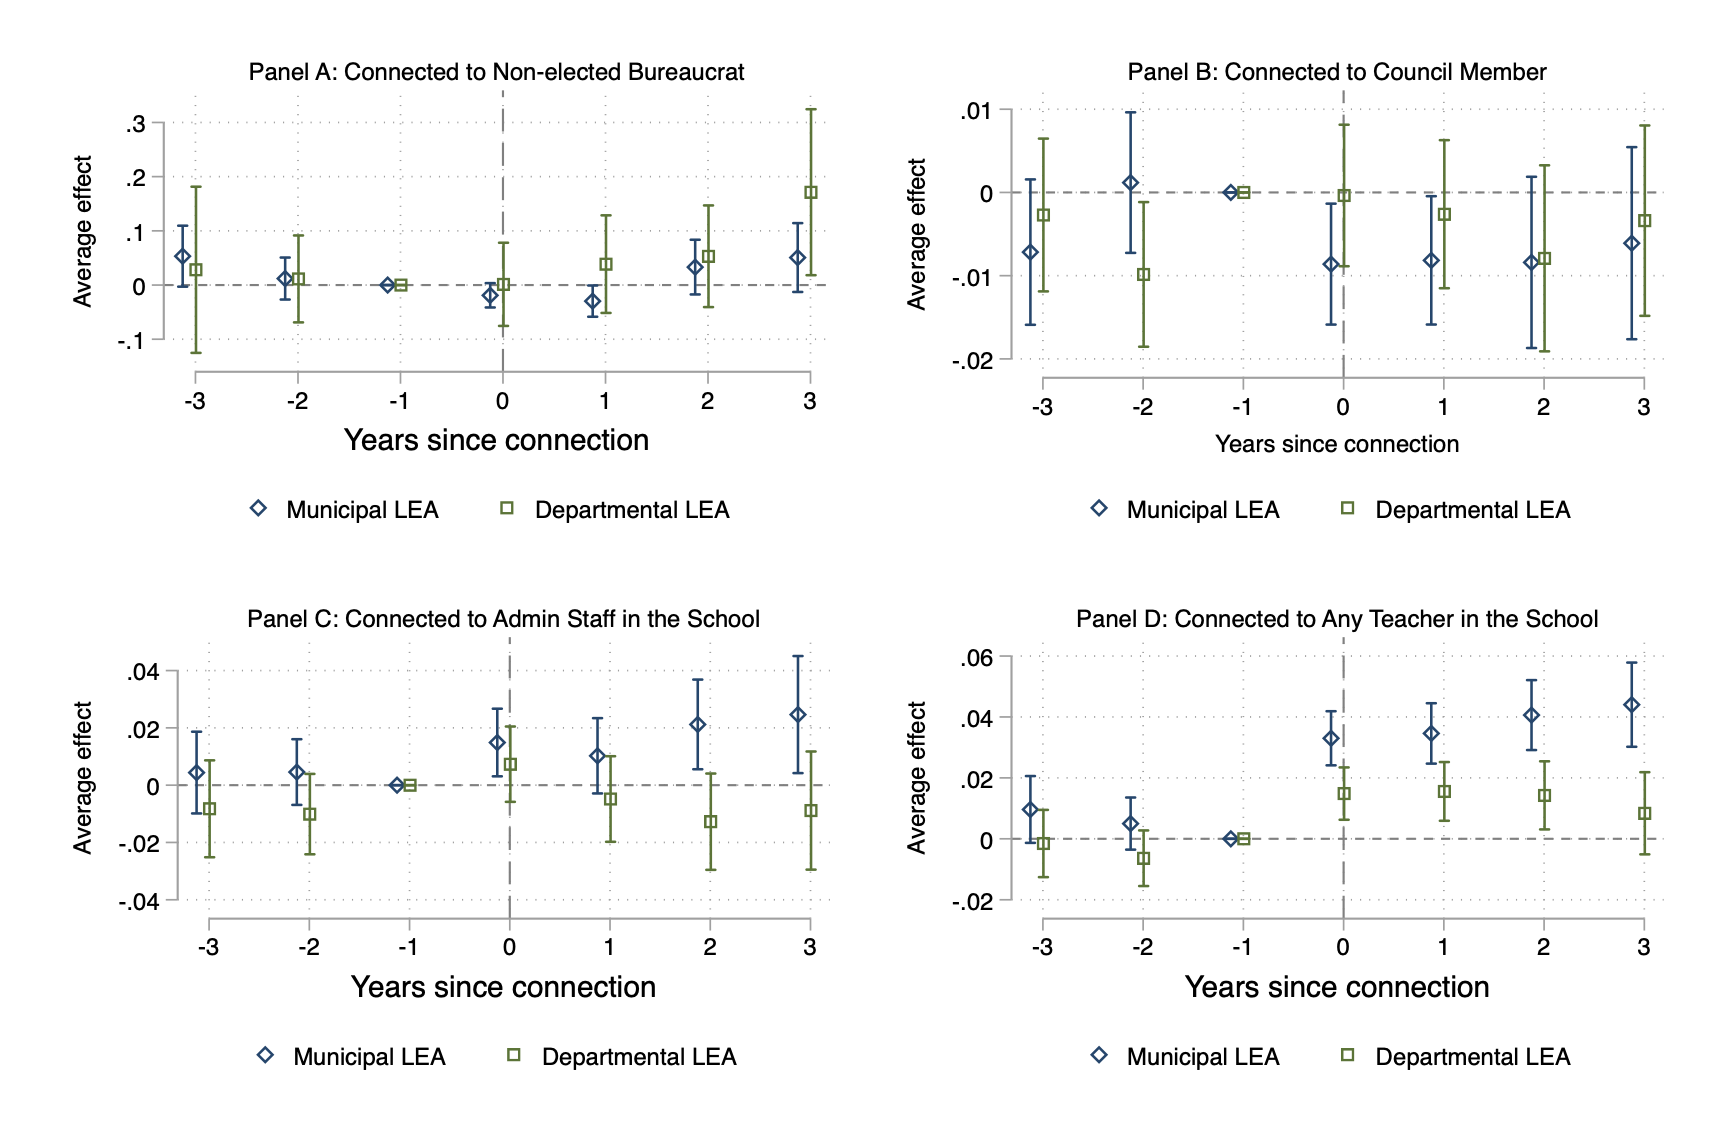
\includegraphics[width = 15cm, height = 12cm]{Figures/heteregoneus_LEA.png}
    \fnote{Source: Ministry of National Education of Colombia and \cite{Riano2021}. 
    LEA stands for local education authority. The municipal LEAs are only responsible for the provision of education in their own municipality, while the departmental LEAs are responsible of the provision in all municipalities in the department that do not have their own LEA.}
\end{figure}

\begin{figure}[H]
   \caption{Event study of having a family connection to a teacher in the school by teacher characteristics}
   \label{fig:event_study_teacher}
    \centering
    \includegraphics[width = 15cm, height = 12cm]{Figures/heteregoneus_teacher.png}
    \fnote{Source: Ministry of National Education of Colombia and \cite{Riano2021}}
\end{figure}

\begin{figure}[H]
   \caption{Event study of having a family connection to a non-elected bureaucrat on being a secondary public school teacher}
   \label{fig:entering}
    \centering
    \includegraphics[width = 15cm, height = 12cm]{Figures/entering_Teaching_career.png}
    \fnote{Source: Ministry of National Education of Colombia and \cite{Riano2021}}
\end{figure}

%%%%%%%%%%%%%%
%%% TABLES %%% 
%%%%%%%%%%%%%%


\newpage
\section*{Tables}

\begin{table}[H]
\renewcommand*{\arraystretch}{1.2}
\scalebox{0.8}{
\begin{threeparttable}
\centering
\caption{Teacher characteristics by connectedness and connection type}
\label{table:tab1}
\begin{tabular}{lccccccc}
\hline  & \multicolumn{3}{c}{Connected} & \multicolumn{3}{c}{Not Connected} & \\
 & N & Mean & SD & N & Mean & SD & Diff\\
\hline \multicolumn{8}{l}{\textit{Panel A: Connection to a Non-elected Bureaucrat}} \\
Female & 1,325 & 0.494 & 0.500 & 500,571 & 0.558 & 0.497 & -0.065***\\
Age & 1,325 & 44.653 & 9.530 & 500,500 & 45.683 & 10.192 & -1.030***\\
Postgrad degree & 1,325 & 0.454 & 0.498 & 500,571 & 0.369 & 0.482 & 0.086***\\
Temporary contract & 1,325 & 0.165 & 0.371 & 500,571 & 0.175 & 0.380 & -0.011\\
Years of experience & 1,325 & 12.273 & 10.517 & 500,435 & 13.985 & 11.291 & -1.711***\\
Students test score & 1,325 & 48.629 & 5.201 & 500,571 & 49.417 & 4.457 & -0.788***\\
Merit exam test score & 806 & 62.867 & 8.479 & 297,987 & 60.866 & 7.940 & 2.001***\\
\\
 \multicolumn{8}{l}{\textit{Panel B: Connection to a Council Member}} \\
Female & 143,010 & 0.565 & 0.496 & 358,886 & 0.555 & 0.497 & 0.010***\\
Age & 142,993 & 45.941 & 10.028 & 358,832 & 45.577 & 10.253 & 0.364***\\
Postgrad degree & 143,010 & 0.372 & 0.483 & 358,886 & 0.368 & 0.482 & 0.004***\\
Temporary contract & 143,010 & 0.152 & 0.359 & 358,886 & 0.185 & 0.388 & -0.033***\\
Years of experience & 142,972 & 14.330 & 11.286 & 358,788 & 13.841 & 11.288 & 0.490***\\
Students test score & 143,010 & 49.585 & 4.531 & 358,886 & 49.347 & 4.429 & 0.239***\\
Merit exam test score & 83,025 & 61.555 & 7.590 & 215,768 & 60.608 & 8.058 & 0.948***\\
\\
\multicolumn{8}{l}{\textit{Panel C: Connection to Administrative Staff in the School}} \\
 Female & 34,003 & 0.556 & 0.497 & 467,893 & 0.558 & 0.497 & -0.002\\
Age & 33,997 & 46.811 & 9.962 & 467,828 & 45.598 & 10.202 & 1.213***\\
Postgrad degree & 34,003 & 0.398 & 0.490 & 467,893 & 0.367 & 0.482 & 0.032***\\
Temporary contract & 34,003 & 0.137 & 0.343 & 467,893 & 0.178 & 0.383 & -0.042***\\
Years of experience & 33,995 & 15.718 & 11.565 & 467,765 & 13.854 & 11.259 & 1.864***\\
Students test score & 34,003 & 49.412 & 4.619 & 467,893 & 49.415 & 4.448 & -0.003\\
Merit exam test score & 17,809 & 61.608 & 7.633 & 280,984 & 60.824 & 7.959 & 0.784***\\
\\
 \multicolumn{8}{l}{\textit{Panel D: Connection to Any Teacher in the School}} \\
  Female & 287,736 & 0.563 & 0.496 & 214,160 & 0.551 & 0.497 & 0.013***\\
Age & 287,694 & 46.111 & 10.079 & 214,131 & 45.102 & 10.311 & 1.010***\\
Postgrad degree & 287,736 & 0.383 & 0.486 & 214,160 & 0.349 & 0.477 & 0.034***\\
Temporary contract & 287,736 & 0.155 & 0.362 & 214,160 & 0.202 & 0.402 & -0.047***\\
Years of experience & 287,653 & 14.692 & 11.401 & 214,107 & 13.023 & 11.065 & 1.669***\\
Students test score & 287,736 & 49.616 & 4.476 & 214,160 & 49.144 & 4.424 & 0.472***\\
Merit exam test score & 164,362 & 61.235 & 7.831 & 134,431 & 60.426 & 8.054 & 0.808***\\
\hline\end{tabular}\\

\begin{tablenotes}
\footnotesize
\item \textit{Notes:} Observations at the teacher-year level. ***, **, and * indicate significance at the 1, 5, and 10 percent critical level. \\
Source: Ministry of National Education of Colombia and \cite{Riano2021}
\end{tablenotes}
\end{threeparttable}}
\end{table}


\newpage
\begin{table}[H]
\renewcommand*{\arraystretch}{1.2}
\begin{threeparttable}
\centering
\caption{Effects of having a family connection on test scores}
\label{table:tab_results}
\setlength{\pdfpagewidth}{8.5in} \setlength{\pdfpageheight}{11in}
\begin{document}
\begin{tabular}{lcccc} \hline
 & \multicolumn{4}{c}{Teacher is family connected to:} \\
 & Bureaucrat & Council member & Admin staff & Any teacher \\
 & (1) & (2) & (3) & (4) \\
  \hline
 &  &  &  &  \\
Test scores   & -0.03106*** & -0.00001 & 0.00354 & 0.02070*** \\
 & (0.01042) & (0.00173) & (0.00300) & (0.00200) \\
 &  &  &  &  \\
Observations & 501,255 & 408,101 & 484,539 & 270,460 \\
Teachers & 109,957 & 88,342 & 106,121 & 58,688 \\
R-squared & 0.851 & 0.846 & 0.849 & 0.822 \\
 &  &  &  &  \\
Year FE & Yes & Yes & Yes & Yes \\
 Teacher FE & Yes & Yes & Yes & Yes \\ \hline
\end{tabular}
\end{document}
\begin{tablenotes}
\footnotesize
\item \textit{Notes:} Observations at the teacher-year level. ***, **, and * indicate significance at the 1, 5, and 10 percent critical level. Standard error clustered at the teacher level in parenthesis. 
\end{tablenotes}
\end{threeparttable}
\end{table}


\begin{table}[H]
\centering
\renewcommand*{\arraystretch}{1.2}
\begin{threeparttable}
\caption{Robustness: Effects of having a family connection on test scores using a balanced panel}
\label{table:results_sample}
\setlength{\pdfpagewidth}{8.5in} \setlength{\pdfpageheight}{11in}
\begin{document}
\begin{tabular}{lcccc} \hline
 & \multicolumn{4}{c}{Teacher is family connected to:} \\
 & Bureaucrat & Council member & Admin staff & Any teacher \\
 & (1) & (2) & (3) & (4) \\
  \hline
 &  &  &  &  \\
Test scores  & -0.02461 & -0.00175 & 0.00161 & 0.01769*** \\
 & (0.01577) & (0.00216) & (0.00378) & (0.00255) \\
 &  &  &  &  \\
Observations & 283,395 & 235,802 & 274,190 & 153,039 \\
Teachers & 47,241 & 39,306 & 45,706 & 25,511 \\
R-squared & 0.845 & 0.842 & 0.843 & 0.817 \\
 &  &  &  &  \\
Year FE & Yes & Yes & Yes & Yes \\
 Teacher FE & Yes & Yes & Yes & Yes \\ \hline
\end{tabular}
\end{document}
\begin{tablenotes}
\footnotesize
\item \textit{Notes:} Observations at the teacher-year level. ***, **, and * indicate significance at the 1, 5, and 10 percent critical level. Standard error clustered at the teacher level in parenthesis. 
\end{tablenotes}
\end{threeparttable}
\end{table}



\newpage
\begin{table}[H]
\centering
\renewcommand*{\arraystretch}{1.2}
\begin{threeparttable}
\caption{Robustness: Effects of having a family connection on test scores without teachers with common surnames}
\label{table:robust1}
\setlength{\pdfpagewidth}{8.5in} \setlength{\pdfpageheight}{11in}
\begin{document}
\begin{tabular}{lccc} \hline
 & \multicolumn{3}{c}{Teacher is family connected to:} \\
  & Council member & Admin staff & Any teacher \\
 & (1) & (2) & (3) \\
  \hline
  &  &  &  \\
Test scores & -0.00298 & 0.00430 & 0.02144*** \\
 & (0.00225) & (0.00428) & (0.00235) \\
 &  &  &  \\
Observations & 306,522 & 341,892 & 222,223 \\
Teachers & 66,599 & 74,980 & 48,342 \\
R-squared & 0.849 & 0.851 & 0.829 \\
 &  &  &  \\
Year FE & Yes & Yes & Yes \\
 Teacher FE & Yes & Yes & Yes \\ \hline
\end{tabular}
\end{document}


\begin{tablenotes}
\footnotesize
\item \textit{Notes:} Observations at the teacher-year level. ***, **, and * indicate significance at the 1, 5, and 10 percent critical level. Standard error clustered at the teacher level in parenthesis. 
\end{tablenotes}
\end{threeparttable}
\end{table}

\newpage
\begin{table}[H]
\centering
\renewcommand*{\arraystretch}{1.2}
\begin{threeparttable}
\caption{Robustness checks: Effects of having a family connection on test scores by level of conectedness}
\label{table:robust2}
\setlength{\pdfpagewidth}{8.5in} \setlength{\pdfpageheight}{11in}
\begin{document}
\begin{tabular}{lccc} \hline
 & \multicolumn{3}{c}{Number of extra family connections to:} \\
  & Council member & Admin staff & Any teacher \\
 & (1) & (2) & (3) \\
  \hline
  &  &  &  \\
Test scores & -0.00000 & 0.00000 & 0.01192*** \\
 & (0.00134) & (0.00266) & (0.00133) \\
 &  &  &  \\
Observations & 407,115 & 484,539 & 270,460 \\
Teachers & 88,106 & 106,121 & 58,688 \\
R-squared & 0.846 & 0.849 & 0.822 \\
 &  &  &  \\
Year FE & Yes & Yes & Yes \\
 Teacher FE & Yes & Yes & Yes \\ \hline
\end{tabular}
\end{document}

\begin{tablenotes}
\footnotesize
\item \textit{Notes:} Observations at the teacher-year level. ***, **, and * indicate significance at the 1, 5, and 10 percent critical level. Standard error clustered at the teacher level in parenthesis. 
\end{tablenotes}
\end{threeparttable}
\end{table}

\end{document}
